\chapter{Background} \label{chp:background}

    In recent years, access to low Earth orbit has been made much cheaper by new private companies. To access objectives deeper in space, including rapid transit of humans to Mars, the development of novel propulsion technologies is necessary. 
    
    The concept of laser-thermal propulsion (LTP) was first suggested by \textcite{kantrowitzRelevanceSpace1971} as a way to decrease launch costs and continues to be of interest. This method of propulsion uses a ground- or space-based laser to heat a gas on a spacecraft, which is then expelled out of a nozzle at the exhaust velocity to generate the required thrust.

    In a conventional chemical rocket engine, the energy source is the oxidizer and the fuel, which are reacted together to release energy. They are transported with the rocket and set the temperature of the combustion reaction (typically \qtyrange{2000}{3000}{K}), which is directly related to the exhaust velocity.
    
    Separating the power source used for propulsion (here, the laser) from the spacecraft itself allows crucial weight savings, either increasing the payload mass fraction or decreasing transit time. Using a laser also allows for much greater thrust chamber temperatures than chemical propulsion, as the temperature of these plasmas is typically \qtyrange{15000}{20000}{K}. This gives in turn higher exhaust velocities. This propulsion method could therefore be an order of magnitude more efficient than our current rocket engines, if certain engineering problems can be solved.

    % Discussion on inverse Bremsstralung

    This thesis will focus on the second challenge, as well as constructing a proof of concept 
    
    % , if certain engineering problems can be solved. The main question that remains is how to absorb as much laser energy as possible 

    Increasing the amount of energy deposited by the laser into the working gas remains a topic of active research and is a significant hurdle for the operational use of LTP.

        [Graph of energy loss here (similar but not exactly same as Emmanuel's)]

        The two main conversion efficiencies are:
        \begin{enumerate}
            \item Absorption of the laser energy by the plasma
            \item Heat transfer from the plasma to the working gas (e.g. propellant)
        \end{enumerate}

    As the efficencies chosen are different from source to source, these efficencies will be defined where applicable.

    \subsection{Literature review [structure like this? Put background in intro?]}
    \begin{figure}[h]
        \centering
        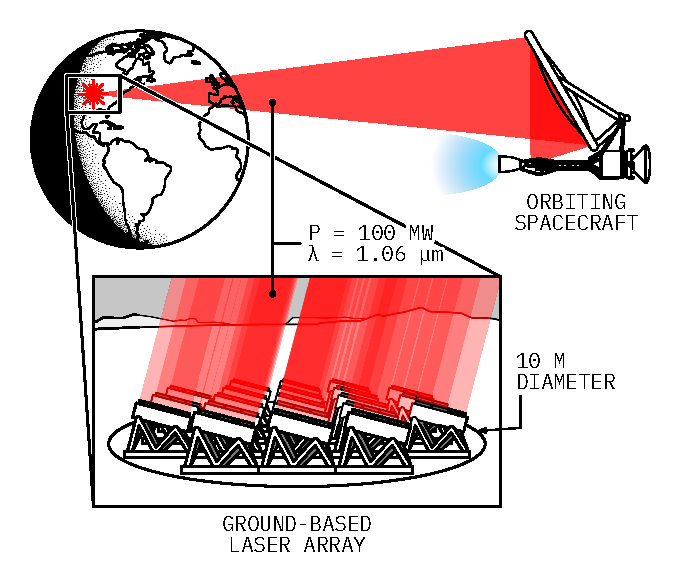
\includegraphics[width=0.35\textwidth]{assets/2 background/ltp_architecture.pdf}
        \caption{LTP architecture (\textcite{duplayArgonLaserPlasmaThruster2024a})}
        \label{fig:LTP architecture}
    \end{figure}

    \begin{figure}[h]
        \centering
        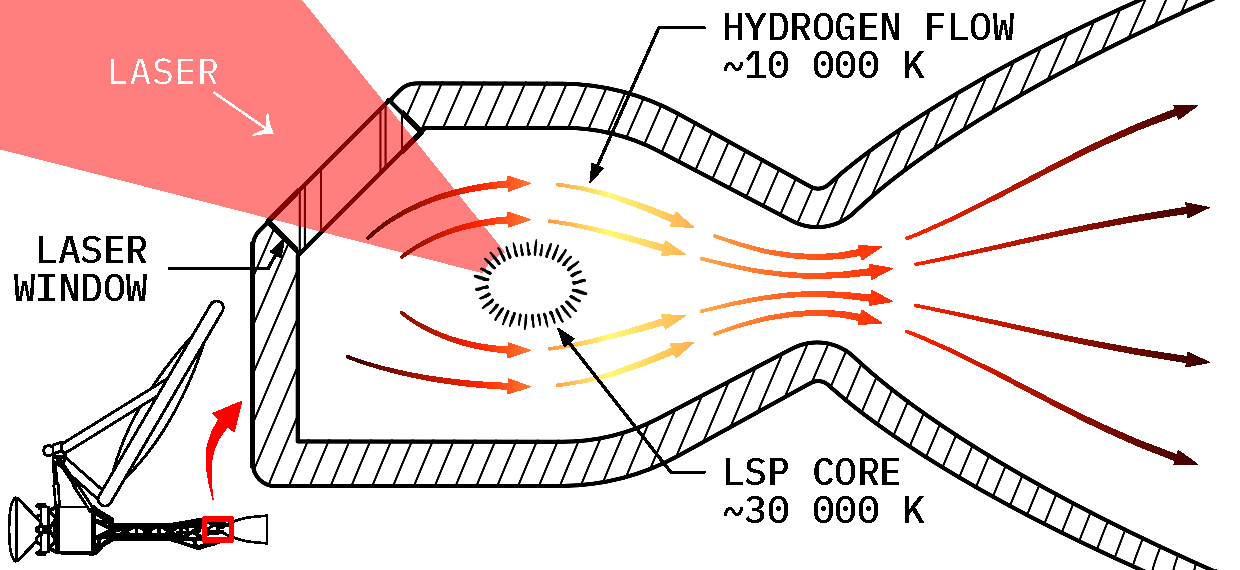
\includegraphics[width=0.35\textwidth]{assets/2 background/chamber.pdf}
        \caption{Overview of LTP system (\textcite{duplayArgonLaserPlasmaThruster2024a})}
        \label{fig:Keefer apparatus}
    \end{figure}
    
    %Russian work: 1960s-2000s?

    The experimental basis of this means of propulsion was developed by \textcite{generalovContinuousOpticalDischarge1970} in 1970. For the first time, an LSP was generated with a \qty{150}{W} \ce{CO2} laser operation at \qty{10.6}{μm} wavelength. In this case, the LSP was ignited by a second, \qty{10}{kW} pulsed \ce{CO2} laser.
    
    Most studies to date have used \ce{CO2} lasers with a wavelength \qty{10.6}{μm}. However, these concepts were limited by a short focusing range due to their long laser wavelength. This relegated them to ground-to-orbit launch. High power fiber lasers emitting near 1 μm have recently become readily available. Being able to beam energy to low earth orbit, fiber lasers make laser propulsion more feasible.

    [move the following citations under section 2.1 Energy deposition:]
    
    %American work: 1970s-1990s?

        Work was done under a NASA grant in the mid-1970s by \textcite{shojiLaserheatedRocketThruster1977,shojiPerformanceHeatTransfer1976a} to design a small-scale \qty{10}{kW} and full-scale \qty{5000}{kW} LTP engine. 
        
        Carbon-seeded hydrogen was used to capture the plasma's radiation, which was mostly in the UV wavelength 
        
        
        
        \qty{19}{\%} of the laser power was lost by radiation in the \qty{10}{kW}. 
        
        The \qty{5000}{kW} thruster loses \qty{4.5}{\%} of laser power by radiation, 



        \begin{figure}[h]
            \centering
            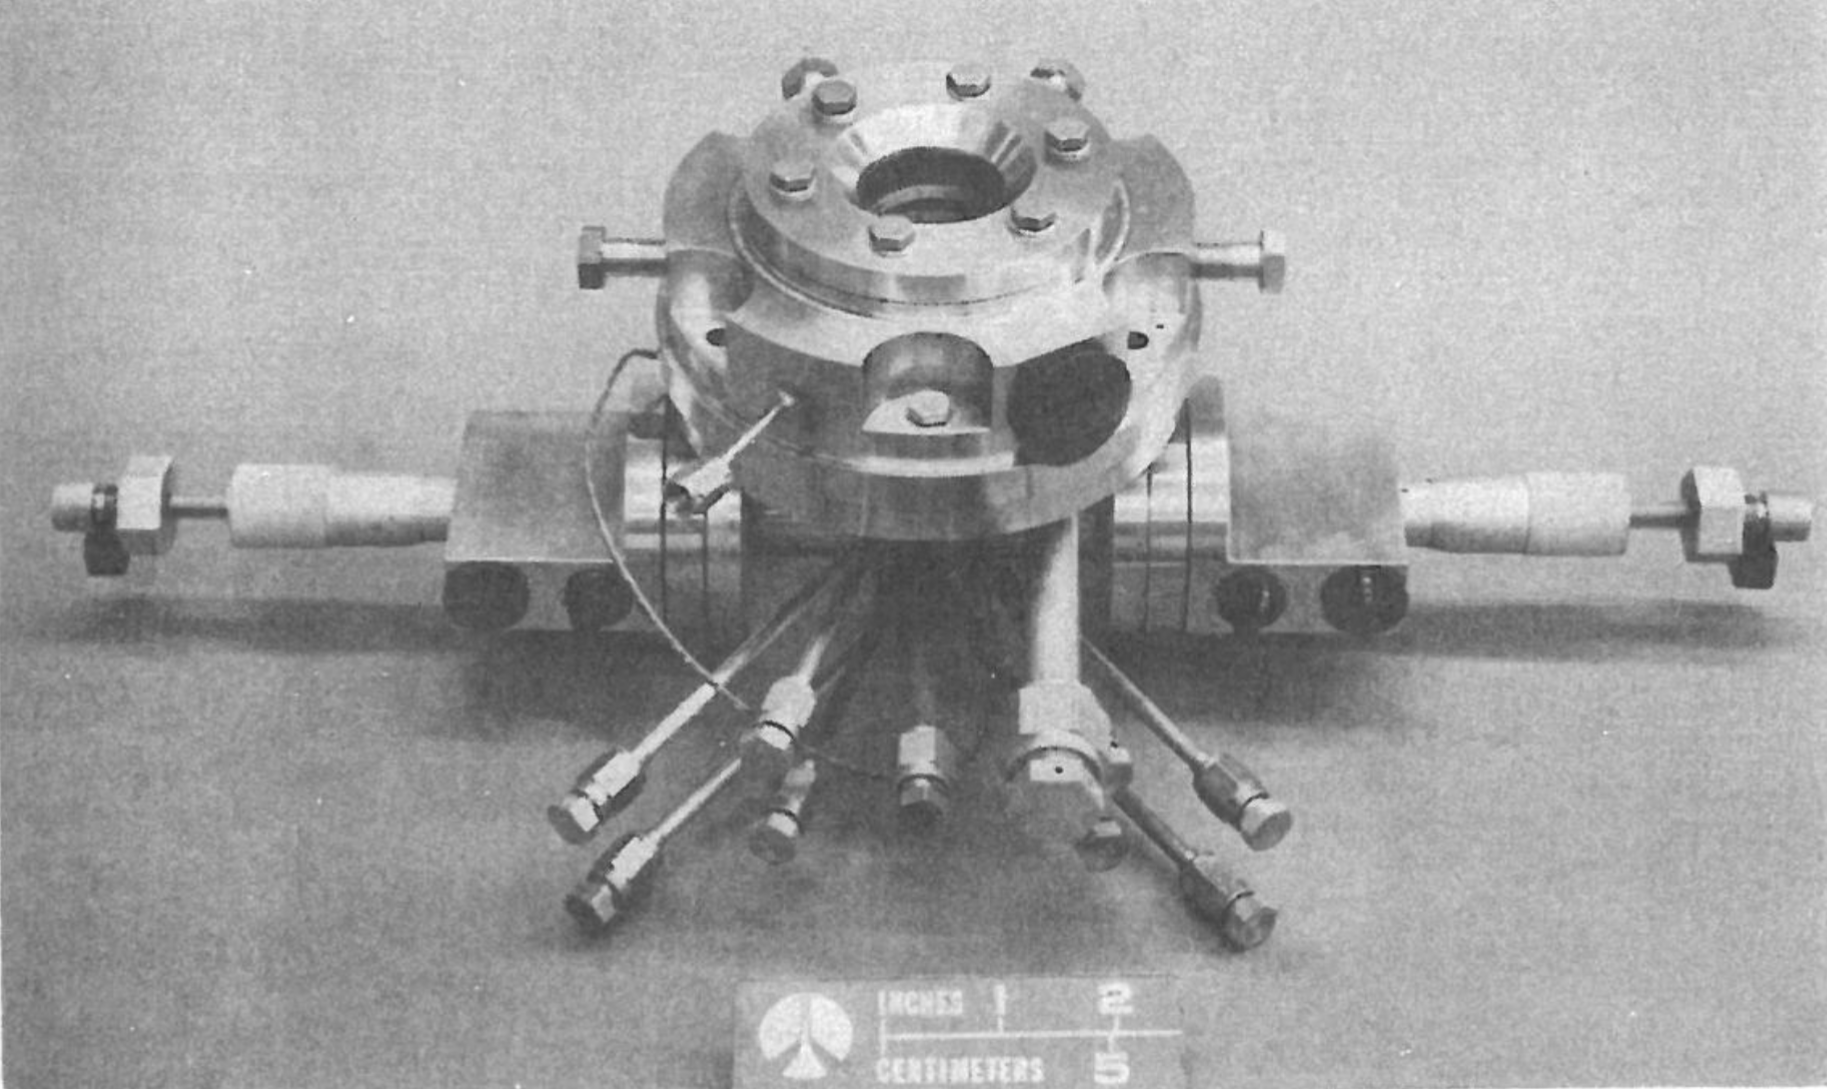
\includegraphics[width=\textwidth]{assets/2 background/Shoji_assy.png}
            \caption{\qty{10}{kW} thruster from \textcite{shojiPerformanceHeatTransfer1976a}}
            \label{fig:Shoji apparatus}
        \end{figure}

        \begin{figure}[h]
            \centering
            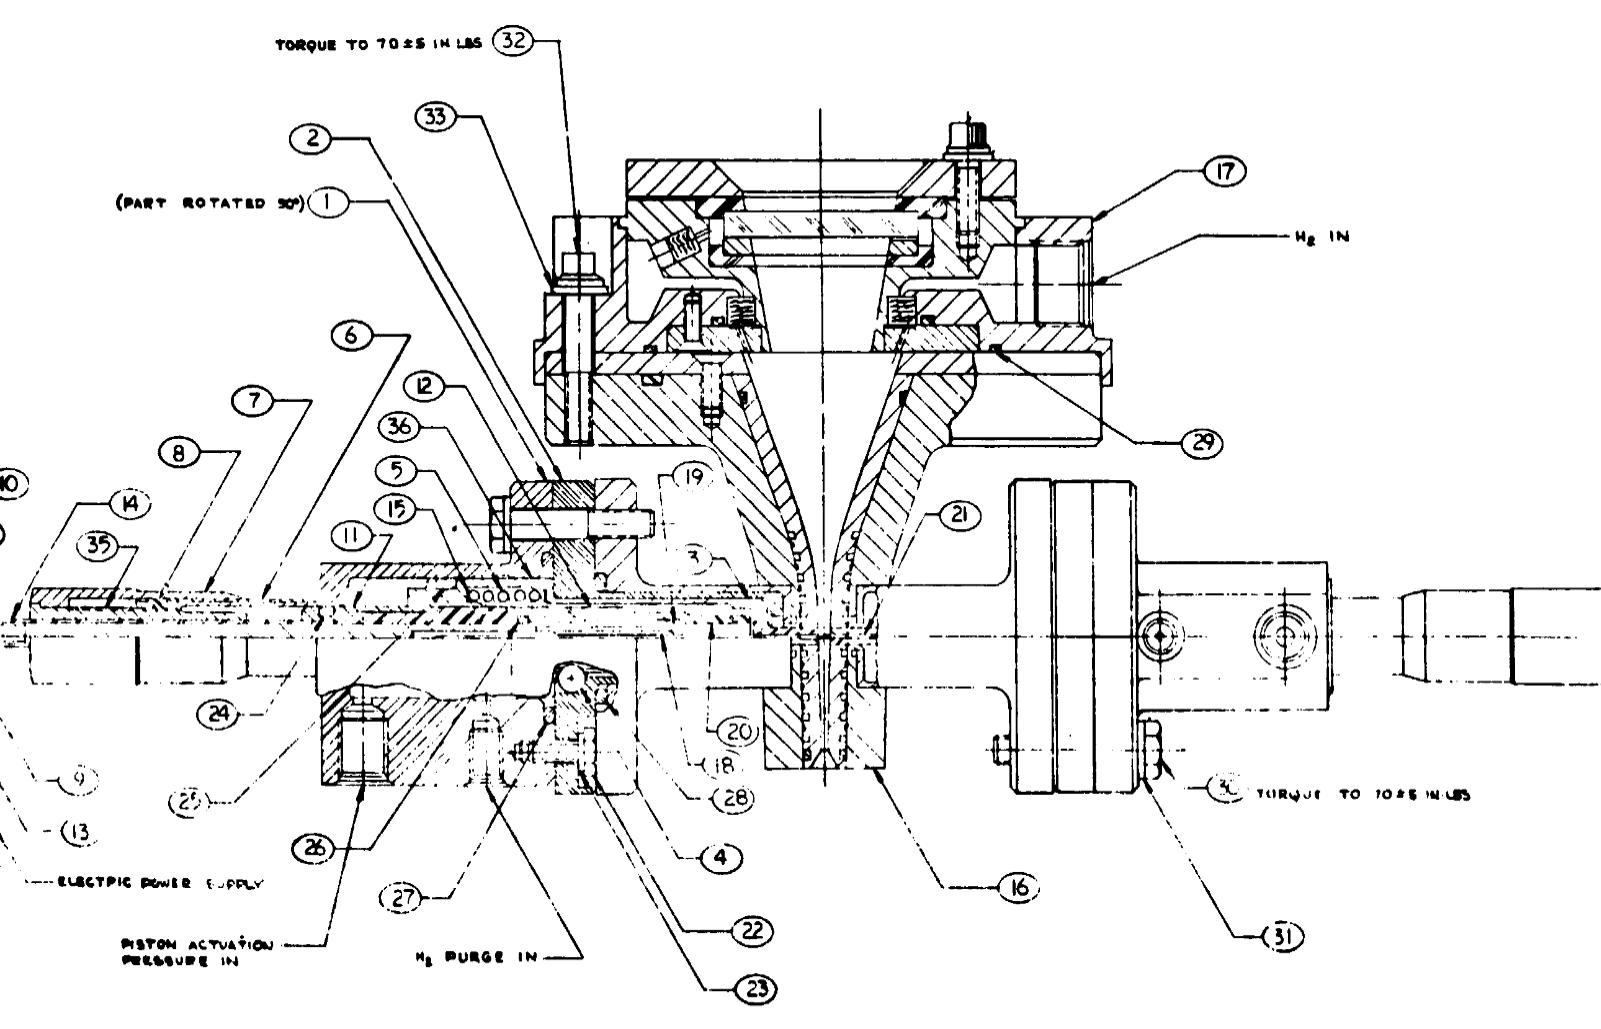
\includegraphics[width=\textwidth]{assets/2 background/Shoji cross-section.png}
            \caption{Cross-section drawing of \qty{10}{kW} thruster from \textcite{shojiLaserheatedRocketThruster1977}}
            \label{fig:Shoji cross-section}
        \end{figure}

        The \qty{10}{kW} prototype (\autoref{fig:Shoji apparatus}) was built and delivered to NASA at the conclusion of the grant.


        
        

        Much work on the topic was done in the 1980s. \textcite{keeferPowerAbsorptionLasersustained1986a} studied LSP in a forced convective flow environment. Using a \qty{1.5}{kW} \ce{CO2} laser with power levels of \qtyrange{360}{840}{W} and pressures of \qtyrange{1.3}{2.3}{atm}, with varying flow velocities, the temperature field of the plasma was measured. From the temperature field, and assuming local thermodynamic equilibrium, the power absorbed by the plasma and the power radiated from it can be calculated.

        \begin{figure}[h]
            \centering
            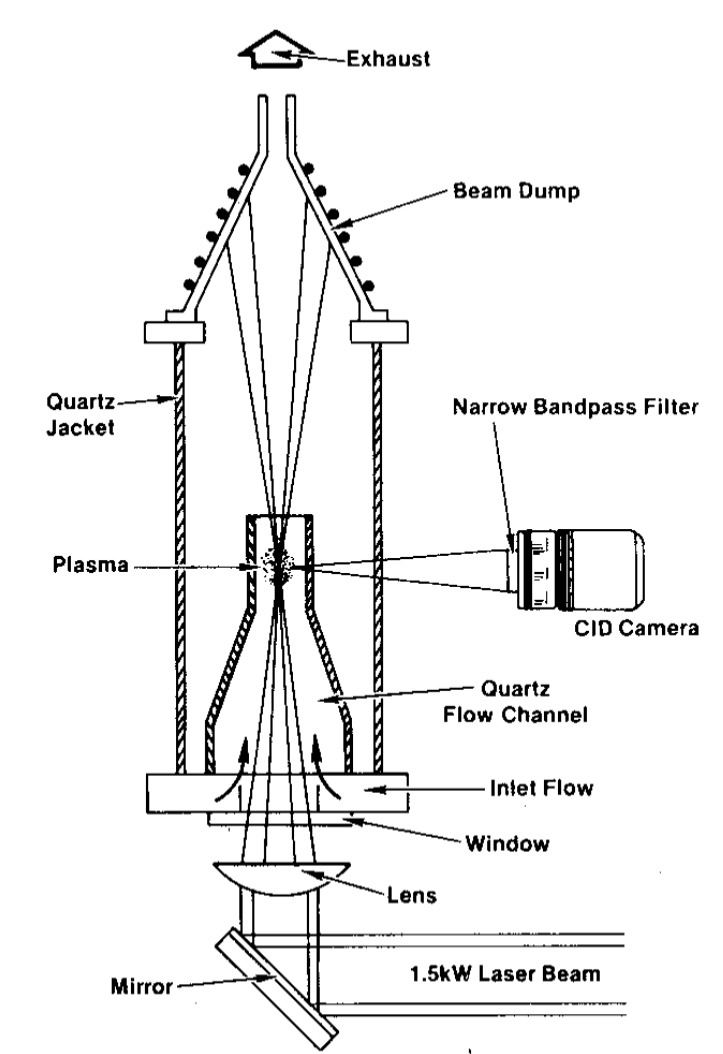
\includegraphics[width=0.35\textwidth]{assets/2 background/UTSI (Keefer) Apparatus.png}
            \caption{Experimental apparatus from \textcite{keeferPowerAbsorptionLasersustained1986a}}
            \label{fig:Keefer apparatus}
        \end{figure}
        
        \autoref{fig:Keefer apparatus} shows the apparatus used for these measurements. An inner quartz flow channel contains the plasma, while an outer quartz jacket contains the pressure. Flowing argon comes in from the bottom and into the flow channel. The plasma is initiated by laser heating of a tungsten rod, which was removed after ignition. Downstream, a water-cooled copper beam dump absorbs the laser energy and cools the heated argon flow.

        \Citeauthor{keeferPowerAbsorptionLasersustained1986a} determined that [PUT PERCENTAGES HERE]

        In parallel, a group from the University of Illinois [say this differently?], reported absorption approaching \qty{80}{\%} and thermal efficiency[...]

        \begin{figure}[h]
            \centering
            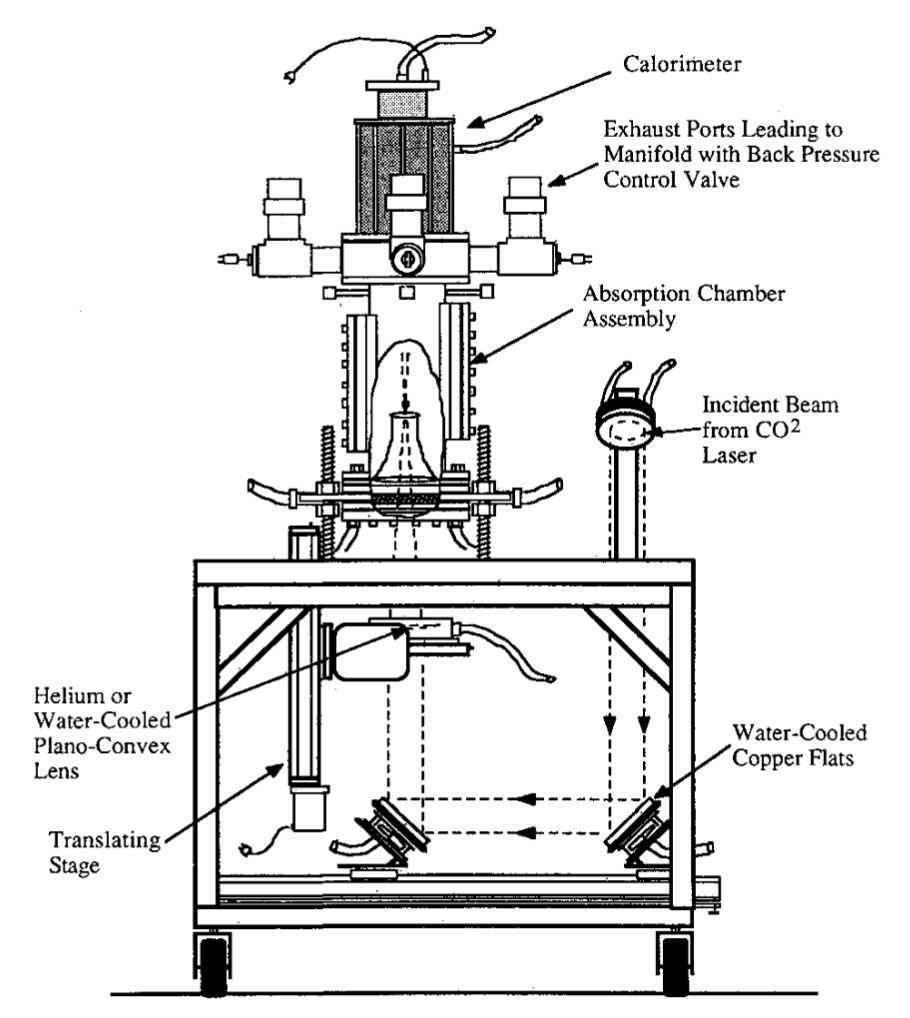
\includegraphics[width=0.35\textwidth]{assets/2 background/Illinois (Krier) Apparatus.png}
            \caption{Experimental apparatus from \textcite{zerkleLasersustainedArgonPlasmas1990}}
            \label{fig:Krier apparatus}
        \end{figure}

        In their later work in 1990, \textcite{zerkleLasersustainedArgonPlasmas1990}, reported absorption from \qtyrange{55}{97}{\%} and thermal efficiency from \qtyrange{11}{46}{\%}. [continue this review, define "thermal efficiency"]

        %LTP research slowed down with the end of high-power laser weapon research in the early 1990s.

        Thrusters with higher laser powers were experimented with by \textcite{blackLaserPropulsion10kW1995}, with a \qty{10}{kW} \ce{CO2} laser. Both argon and hydrogen were used.

        In this study, a preliminary design for a \qty{100}{kW} thruster was presented, with a predicted specific impulse of \qty{1000}{s}, thrust of \qty{4.5}{N} and a conversion efficiency of \qty{80}{\%}.

    %Japanese work: 1980s-2020s?

        In the early 2000s, \textcite{toyodaThrustPerformanceCW2002} built and tested two different thruster models, presented in \autoref{fig:Toyoda apparatus}. These thrusters, using argon or nitrogen heated by LSP, were powered by a \qty{2}{kW} \ce{CO2} laser. The LSPs were ignited by a retractable tungsten rod at the laser's focus. Thrust measurements were done both in atmospheric pressure and in vacuum. This comparative study showed that confining the plasma into a smaller chamber increased heat transfer and therefore, efficiency.
        
        \textcite{toyodaThrustPerformanceCW2002} defines the 'energy conversion efficency' as the amount of laser power that is converted into usable kinetic energy for thrust and is calculated as:

        \[ n_e = F^2 - \frac{F^2_{cold}}{2 \dot{m} P}\]

        Where $F$ is the thrust with laser on, $F_{cold}$ is the cold flow thrust (laser off) and $P$ is incident laser power.

        An energy conversion efficiency of 37\% and an $I_{sp}$ of \qty{113}{s}, the highest recorded, were measured with the second model \autoref{fig:Toyoda apparatus} in vacuum with argon propellant. The pressure ratio, defined as the chamber pressure divided by the nozzle exit pressure, was 420. A water cooling system measured heat loss to the walls to be 55\% of incident laser power, with a final 8\% being 'other loss'. Heat loss to the walls was expected to be recycled with regenerative cooling in a real-world application.

        \begin{figure}[h]
            \centering
            \begin{subfigure}[t]{0.45\textwidth}
                \centering
                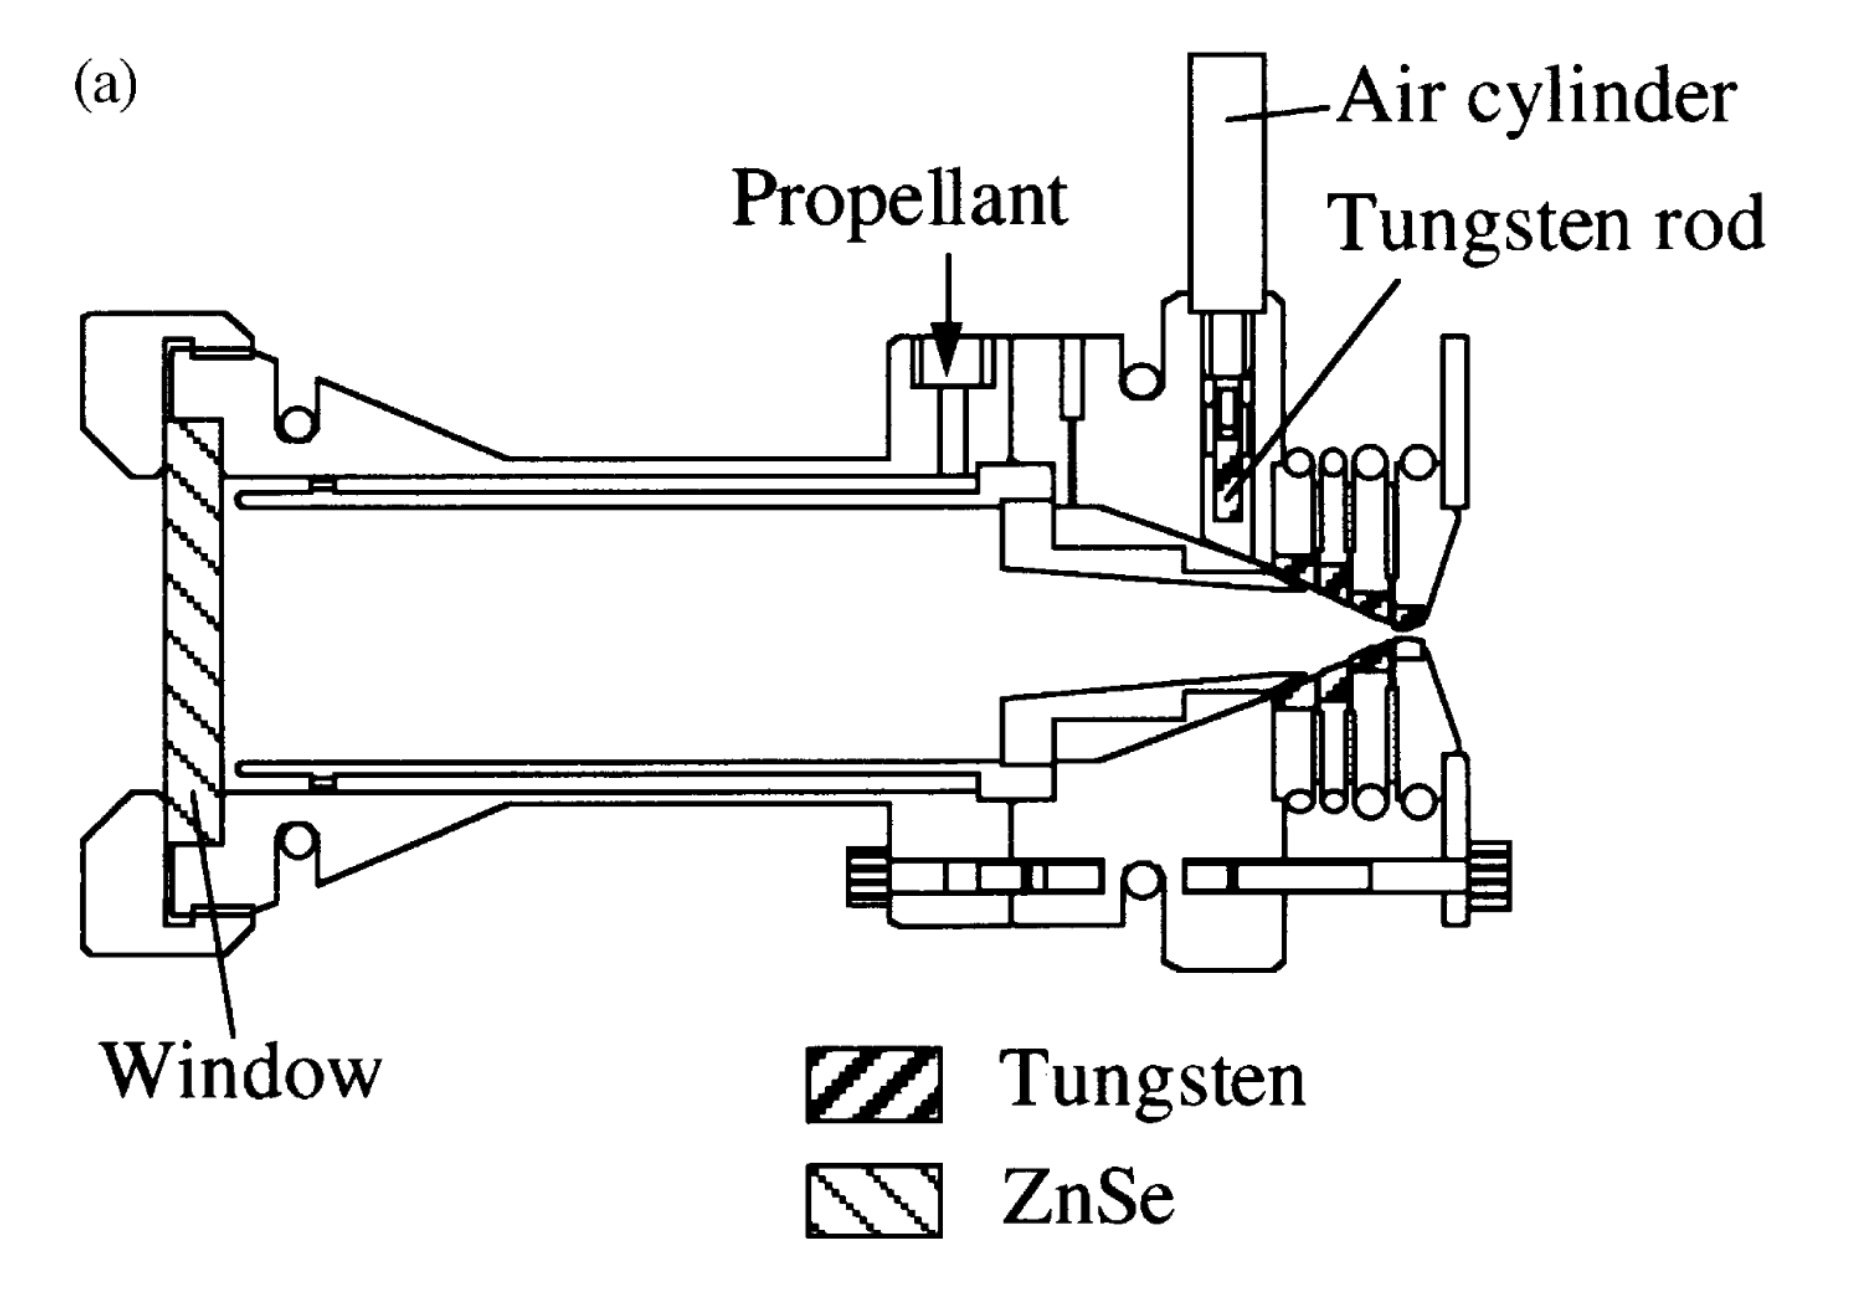
\includegraphics[width=0.35\textwidth]{assets/2 background/Toyoda apparatus model 1.jpg}
                \caption{Model I}
                \label{fig:Toyoda apparatus 1}
            \end{subfigure}
            \hfill
            \begin{subfigure}[t]{0.45\textwidth}
                \centering
                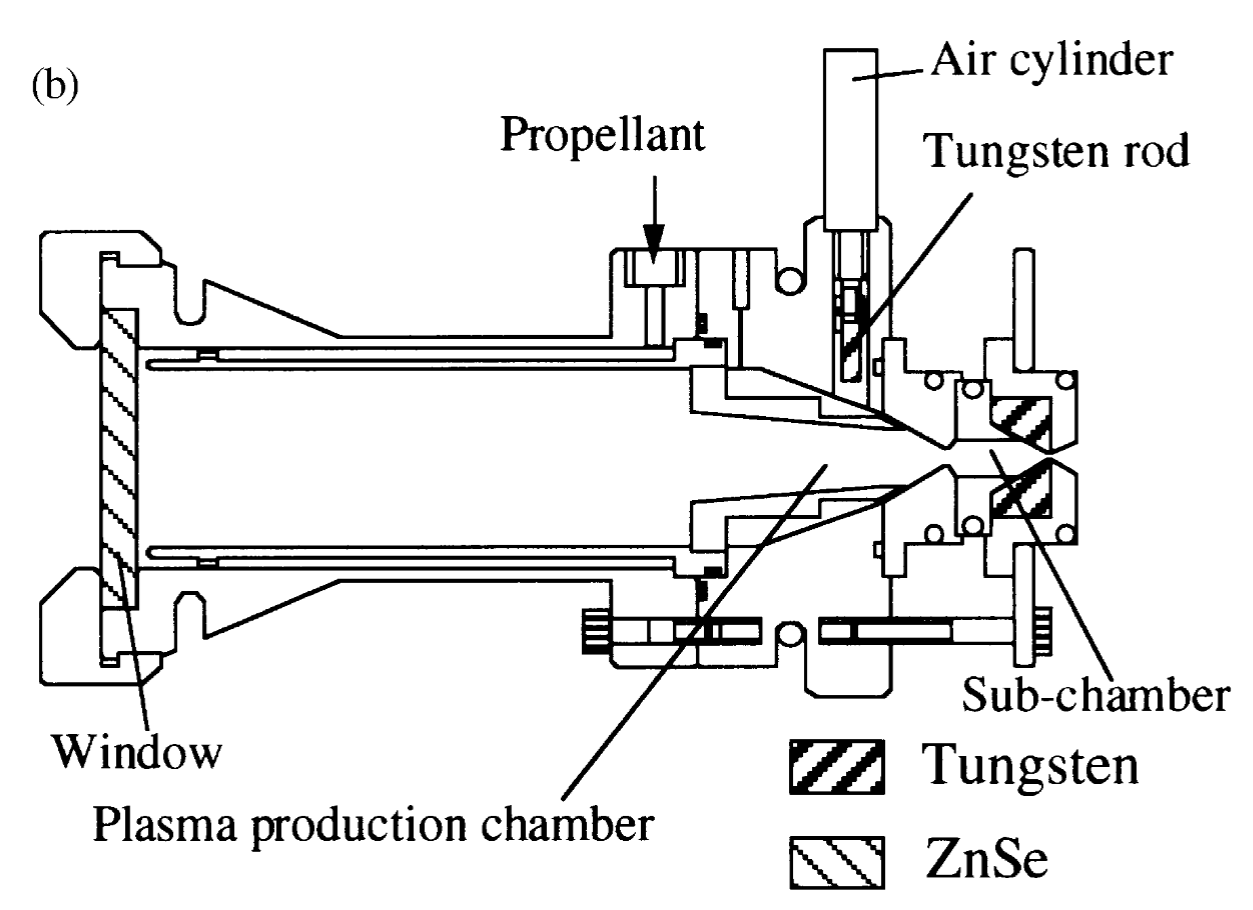
\includegraphics[width=0.35\textwidth]{assets/2 background/Toyoda Apparatus model 2.png}
                \caption{Model II}
                \label{fig:Toyoda apparatus 2}
            \end{subfigure}
            \caption{Two thruster models from \textcite{toyodaThrustPerformanceCW2002}}
        \end{figure}

        %More recently, work by Matsui [look into his work here https://scholar.google.com/citations?view_op=list_works&hl=fr&hl=fr&user=eeEONzQAAAAJ&sortby=pubdate]

    %Chinese work: 2020s?

        \textcite{luCharacteristicDiagnosticsLaserStabilized2022a} investigated LSP for lighting applictions instead of propulsion. Therefore, an emphasis was made on spectroscopy measurements. A \qty{300}{W} fiber laser at a wavelength of \qty{1080}{nm} was focused to a \qty{50}{um} diameter spot in a high pressure chamber.
        
        \begin{figure}[h]
            \centering
            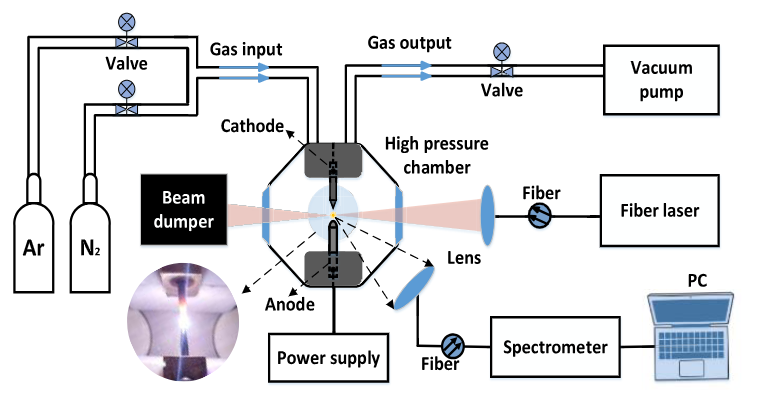
\includegraphics[width=0.35\textwidth]{assets/2 background/Lu apparatus.png}
            \caption{Experimental setup from \textcite{luCharacteristicDiagnosticsLaserStabilized2022a}}
            \label{fig:Lu apparatus}
        \end{figure}

        Argon pressures between \qtyrange{10}{20}{bar} were used. \ce{N2} was later added between \qtyrange{0.1}{1.0}{\%}. A lower ignition power (\qty{117}{W}) than other studies was achieved at \qty{20}{bar}. This was attributed to the smaller focus delivering a higher photon flux.
        
        As expected, increasing the laser power or the gas pressure were found to increase the radiation intensity of the LSP. However, adding \ce{N2} reduced both the electron temperature and electron density of the LSP, reducing its radiation intensity.

    %Canadian work: 2020s

        This thesis builds directly upon \textcite{duplayArgonLaserPlasmaThruster2024a}'s Master's thesis. 



       

        

        % Lubin papers

        % To change/update: Preliminary work done by the McGill Interstellar Flight Experimental Research Group indicated that with the first generation thruster, about \qty{80}{\%} of the laser energy was being absorbed by the plasma, with approximately \qty{15}{\%}    

        Seeding the working gas with another species has been discussed as a way to increase the energy absorption into the working fluid of an LTP engine. Carbon particles have been suggested by [SHOJI, rework these sentences].

        Pure methane and methane-seeded gasses have been experimentally investigated by \textcite{kameiMethaneMethaneXenon2020}. The rationale is similar to carbon particles, as the methane dissociates into hydrogen and carbon with the high temperature of the LSP. A \qty{1.1}{kW} diode laser at a wavelength of \qty{940}{nm} was beamed into a high-pressure chamber fitted with arc ignition electrodes. The gap between these electrodes was \qty{1}{mm}. A CCD type spectrometer recorded emission spectra of the ignition arc discharge and of the LSP. LSPs in three different gasses were attempted: pure methane, methane-argon and methane-xenon.
        
        \begin{figure}[h]
            \centering
            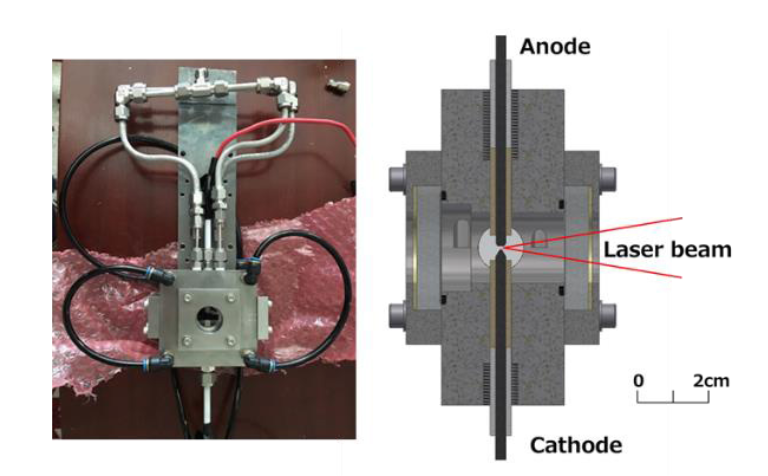
\includegraphics[width=0.35\textwidth]{assets/2 background/Kamei apparatus.png}
            \caption{LSP generation chamber and cross section view from \textcite{kameiMethaneMethaneXenon2020}}
            \label{fig:Kamei}
        \end{figure}

        In methane at \qty{0.1}{MPa}, soot formation between the electrodes prevented LSP ignition. The spectrometer confirmed the dissociation of methane, as line spectra of carbon and hydrogen were observed at the ignition arc. Ignition was also unsucessful in argon-methane with a pressure between \qtyrange{0.1}{0.3}{MPa} and a methane volume fraction between \qtyrange{20}{60}{\%}. 
        
        LSP was successfully generated in methane-xenon, with a lower threshold power (\qty{850}{W}) than in pure xenon. The partial pressure of methane was between \qtyrange{0.02}{0.6}{MPa}, with a partial pressure of xenon of \qty{0.10}{MPa}.

    \section{Summary and direction of work in this thesis}

        \begin{table}[ht] % TODO - update this table. Column is very narrow and difficult to read. If you cannot make it wider, might consider eliminating this column and instead have this information appear as footnotes below the table, which are much easier to read. Also, since many of the entries are the same "Arc discharge ignition", the same footnote can be used over and over.
            \small
            \centering
            \caption{Summary of a selection of past LSP experiments. $\lambda$: wavelength, $P$: maximum laser power, $p$: pressure, $I_\mathrm{sp}$: maximum specific impulse, $F_\mathrm{T}$: maximum thrust}
            \label{tab:pastexp}
            \begin{tabularx}{\textwidth}{@{}>{\small}X<{\raggedright}llrrlrrr>{\footnotesize}X<{\raggedright}@{}}
            \toprule
            {LSP   Facility}                                                           & Year & Laser         & $\lambda$   [\unit{\um}] & $P$ [kW] & Gas                 & $p$   [atm] & $I_\mathrm{sp}$ [s] & $F_\mathrm{T}$   [N] & {Comments}                                                                   \\ \midrule
            \textcite{generalovContinuousOpticalDischarge1970}                                                         & 1970 & \ce{CO_2}                  & 10.60             & 0.15               & \ce{Xe}              & 3.0 - 4.0        &           -             &       -       & First   LSP                                                              \\
            \textcite{keeferPowerAbsorptionLasersustained1986a}         & 1986 & \ce{CO_2}                  & 10.60             & 0.84        & \ce{Ar}              & 1.3   - 2.3      &            -            &       -       & Specialized   laser beam dump integrated within the converging exit nozzle \\
            \textcite{blackLaserPropulsion10kW1995}          & 1995 & \ce{CO_2}                  & 10.60             & 10.00              & \ce{Ar},   \ce{H_2}    & 1.0   - 2.7      & 350                    & 3.00         & \footnote{15:1   expansion ratio nozzle}                                              \\
            \\
            \textcite{toyodaThrustPerformanceCW2002} & 2002 & \ce{CO_2}                  & 10.60             & 2.00               & \ce{Ar},   \ce{N_2}    & 2.0   - 5.5      & 113             & 0.44         & \footnote{Tungsten   rod ignition}                                                    \\
            \textcite{zimakovInteractionNearIRLaser2016}                                                        & 2016 & Fiber                & 1.07              & 1.50        & \ce{Ar},   \ce{Xe}   & 3.0   - 24.7     & -                      & -            & \footnote{Arc   discharge ignition}                                                   \\
            \textcite{matsuiGeneratingConditionsArgon2019}                                                          & 2019 & Fiber &      1.07             &        2.00            &           \ce{Ar}           &          1.0 - 64.2        &            -            &       -       & \footnote{Arc   discharge ignition}                                               \\
            \textcite{luCharacteristicDiagnosticsLaserStabilized2022a}                                                             & 2022 & Fiber                & 1.08              & 0.30      & \ce{Ar},   \ce{N_2} & 9.9   - 19.7     & -                      & -            & \footnote{Arc   discharge ignition}                                                   \\ \bottomrule
            \end{tabularx}
            
        \end{table}

            [Summary of lit review]
            
            The objective of this research project is to test a lab-scale proof-of-concept LTP thruster for interplanetary space flight, using a \qty{1.07}{um} fiber laser. The main objective of the proposed research will be to measure the key performance parameters of this thruster (thrust and specific impulse), as well as characterize the laser-sustained plasma (LSP) heating core inside the thruster. This project will mainly build upon the experimental research started by \textcite{duplayArgonLaserPlasmaThruster2024a}.

            % mention The original contribution of this work ?
